\label{chap:Post-Processing}
% ---------------------------------------------------------------------------
\section{Introduction}
\label{sec:pp-introduction}
% ---------------------------------------------------------------------------

The post-processing framework acts as the analysis and visualization bridge between raw simulation output and the user. Unlike traditional simulator output utilities, this framework provides a unified programmable interface that combines measurement, waveform arithmetic, visualization, and automated analysis within the same simulation environment. It interprets the generated numerical data from the circuit simulator through measurements, mathematical operations, and waveform visualization. This chapter outlines the design, mathematical models, and implementation of this command-driven post-processing system, detailing its architecture, analysis algorithms, software structure, and automated verification strategies.
\section{System Architecture}
\label{sec:pp-architecture}
% ---------------------------------------------------------------------------

The post-processing framework represents the analysis and visualization layer of the simulation environment. After simulation completion, the generated standard SPICE raw file is parsed, reconstructed into waveform data, and processed through measurement, mathematical, and visualization operations.

The overall organization of the post-processing framework is illustrated in Figure~\ref{fig:postprocessing_flow}. The architecture follows a layered pipeline where data moves from the simulator output layer toward analysis and visualization services.

% ---- Architecture Flow Figure ------------------------------------------------
\textsc{\begin{figure}[!ht]
  \centering
  \small
  \setlength{\fboxsep}{5pt}
  \begin{tabular}{ccc}
    \multicolumn{3}{c}{\fbox{\parbox{0.58\textwidth}{\centering \texttt{User}}}}\\[0.1em]
    \multicolumn{3}{c}{$\downarrow$}\\[0.1em]
    \multicolumn{3}{c}{\fbox{\parbox{0.58\textwidth}{\centering \texttt{Command Interface}}}}\\[0.1em]
    \multicolumn{3}{c}{$\downarrow$}\\[0.1em]
    \multicolumn{3}{c}{\fbox{\parbox{0.58\textwidth}{\centering \texttt{Interpreter}}}}\\[0.1em]
    $\swarrow$ & $\downarrow$ & $\searrow$\\[0.1em]
    \fbox{\texttt{MeasEngine}} & \fbox{\texttt{CalcEngine}} & \fbox{\texttt{PlotEngine}}\\[0.1em]
    $\uparrow$ & $\downarrow$ & $\uparrow$\\[0.1em]
    \multicolumn{3}{c}{\fbox{\parbox{0.58\textwidth}{\centering \texttt{WaveformDB}}}}\\[0.1em]
    \multicolumn{3}{c}{$\uparrow$}\\[0.1em]
    \multicolumn{3}{c}{\fbox{\parbox{0.58\textwidth}{\centering \texttt{RawfileReader}}}}\\[0.1em]
    \multicolumn{3}{c}{$\uparrow$}\\[0.1em]
    \multicolumn{3}{c}{\texttt{.raw file}}
  \end{tabular}
  \caption{High-level post-processing data flow and control hierarchy.}
  \label{fig:postprocessing_flow}
\end{figure}}
\newpage
% ---------------------------------------------------------------------------
The framework consists of the following components:

\begin{enumerate}
\item \textbf{RawfileReader} --- Parses the standard SPICE raw file format by extracting metadata from the ASCII header and reconstructing waveform samples from the binary data section.
\item \textbf{WaveformDB} --- Maintains loaded simulation records and provides unified, analysis-type-aware signal lookup.
\item \textbf{Interpreter} --- Tokenises user input and dispatches commands to the appropriate analysis engines.
\item \textbf{MeasEngine} --- Computes numerical characteristics such as maximum value, rise time, frequency, and delay from waveform data.
\item \textbf{CalcEngine} --- Evaluates mathematical expressions over signals and stores derived waveforms for later analysis.
\item \textbf{PlotEngine} --- Generates engineering waveform visualization using \texttt{gnuplot}, including automatic Bode plot generation for AC simulation results.
\end{enumerate}

Overall, the architecture creates a clear separation between simulation data acquisition, waveform management, user interaction, and analysis operations. This modular structure enables reliable extension of the tool with additional measurements, commands, or visualization capabilities.

% ---------------------------------------------------------------------------


\paragraph{Architecture Design Principles.}

The post-processing architecture follows the following design principles:

\begin{itemize}
\item \textbf{Separation of responsibilities:} Each subsystem performs one main task. File parsing, storage, command execution, numerical analysis, and visualization are isolated.
\item \textbf{Extensibility:} The command interface is based on the \texttt{ICommand} abstraction, allowing new commands to be integrated without modifying the interpreter.
\item \textbf{Data reuse:} WaveformDB stores processed simulation results in memory, avoiding repeated parsing operations.
\item \textbf{Analysis independence:} Measurement, calculation, and plotting engines operate independently from the user interface layer.
\end{itemize}
% ---------------------------------------------------------------------------

% ---------------------------------------------------------------------------

% ---------------------------------------------------------------------------
\section{Data Model}
\label{sec:pp-datamodel}
% ---------------------------------------------------------------------------
\subsection{Waveform Representation}

A simulation result is represented as a discrete waveform:

\begin{equation}
W = \{(x_i,y_i)\}_{i=0}^{N-1}
\end{equation}

where $x_i$ represents the independent variable and $y_i$ represents the corresponding waveform sample. For AC analysis, each sample is represented internally using its real and imaginary components.

The independent variable may represent time in transient analysis, frequency in AC analysis, or a swept parameter in DC analysis.

\subsection{\texttt{RawfileReader}}
\label{subsec:rawfile-reader}

The \texttt{RawfileReader} is implemented as a stateless utility component that parses a simulation output
file and returns a fully populated in-memory structure.  The file format
follows standard SPICE output conventions: an ASCII header section describes the
metadata and variable list, followed by a binary data block that
stores all sample values in row-major order.
\newpage
\paragraph{Parsing Algorithm}

Algorithm~\ref{alg:raw-reader} summarizes the main parsing procedure.

\begin{algorithm}[H]
\caption{ReadRawFile}
\label{alg:raw-reader}
\textbf{Input:} binary \texttt{.raw} file \\
1. Read ASCII header \\
2. Extract simulation metadata \\
3. Detect analysis type \\
4. Allocate waveform vectors \\
5. Parse binary block \\
6. Convert samples \\
7. Return \texttt{RawFile} object
\end{algorithm}

The parsing process consists of two main stages: metadata extraction and binary waveform reconstruction.

\paragraph{Header fields parsed.}
The reader extracts the following fields from the ASCII header:
\begin{itemize}
  \item \texttt{Title} --- a free-text description of the simulation.
  \item \texttt{Date} --- the timestamp written by the simulator.
  \item \texttt{Plotname} --- a keyword that identifies the analysis type
        (\texttt{Transient}, \texttt{AC}, \texttt{DC}, or
        \texttt{Operating Point}).
  \item \texttt{Flags} --- set to \texttt{complex} for AC analyses; absent or
        empty for real analyses.
  \item \texttt{No.\ Variables} --- total number of signals (including the sweep variable).
  \item \texttt{No.\ Points} --- total number of time/frequency steps.
  \item \texttt{Variables} block --- one tab-delimited line per signal giving
        its index, name, and type.
\end{itemize}

\paragraph{Binary data layout and Constraints.}
For \emph{real} analyses the binary section stores doubles in row-major order.
For \emph{complex} AC analyses the sweep variable occupies a single double per
row, while each remaining variable occupies two consecutive doubles
(real part followed by imaginary part). The reader reconstructs the waveform vectors by mapping each binary sample position to the corresponding variable index extracted from the header. Only the \texttt{Binary:} data
section is supported. Signal names are looked up case-insensitively.

\subsection{Waveform Database}
\label{subsec:waveform-db}

The waveform database (\texttt{WaveformDB}) is the central in-memory repository
that maintains all loaded simulation results. The database abstraction avoids direct coupling between file parsing and analysis modules. After loading, all engines operate on a unified waveform representation rather than depending on the original storage format.  Each call to the
\texttt{load} method parses one raw file and appends a \emph{plot record}
to an internal list.

\subsection{PlotRecord}
\label{subsec:plotrecord}
Each record carries:
\begin{itemize}
  \item A short \emph{tag} derived automatically from the file stem
        (e.g., \texttt{test\_rc\_TRAN\_0}).
  \item The analysis type: \texttt{OP}, \texttt{DC}, \texttt{TRAN}, or \texttt{AC}.
  \item The X-axis vector and a map of Y signal names to sample vectors.
  \item For AC results, the imaginary column is named with a \texttt{\_im} suffix.
\end{itemize}

\paragraph{Signal look-up order.}
When a command requests a signal by name, the database searches:
\begin{enumerate}
  \item Computed (derived) signals created by the \texttt{calc} command.
  \item Raw records in reverse-load order (most recently loaded first).
  \item Lazy-evaluated complex-accessor wrappers (\texttt{mag(\ldots)},
        \texttt{ph(\ldots)}, \texttt{db(\ldots)}, \texttt{re(\ldots)},
        \texttt{im(\ldots)}).
\end{enumerate}

\section{Command Interface}
\label{sec:command-interface}

\subsection{Grammar}
\label{subsec:command-grammar}

The command-line interface follows a small verb-first grammar. The syntax is
intentionally constrained so that every command can be parsed deterministically
before it is dispatched to a specialised engine.

\begin{itemize}
  \item \textbf{Command Structure:} \texttt{<Verb> <Arguments> <Options>}
  \item \textbf{Plot Command:} \texttt{plot <XAxis> <YSignal>+ <PlotOptions>}
  \item \textbf{Measurement Command:} \texttt{meas <MeasureType> <Signal> [<MeasureArgs>]}
  \item \textbf{Calculation Command:} \texttt{calc <Expression>}
\end{itemize}

The grammar intentionally separates command identification from argument processing, allowing the interpreter to validate command structure before execution.

% ---------------------------------------------------------------------------
\subsection{Execution Modes}
\label{sec:pp-invocation}
% ---------------------------------------------------------------------------

The post-processor is invoked as a standalone executable.  Three modes of
operation are supported:

\begin{description}
  \item[One-shot mode] One or more raw files are given as positional
    arguments followed by a command and its arguments.  The tool loads all
    files, executes the single command, prints the result, and exits.
    Example syntax: \\[0.3em]
    \texttt{\textit{tool} \textit{file.raw} [\textit{file2.raw}~\ldots] \textit{command} [\textit{args}]}

  \item[Interactive mode] Invoked with the \texttt{-i} (or
    \texttt{--interactive}) flag, or with no arguments at all, the tool
    starts a prompt-driven REPL (\texttt{spice>}).  The user may load
    additional files, run any number of commands, and exit by typing
    \texttt{exit}, \texttt{quit}, or \texttt{q}.

  \item[Script mode] Invoked with \texttt{--script \textit{file}}, the
    tool reads commands from a plain-text script file line by line.  Lines
    beginning with \texttt{\#} are treated as comments and skipped.
\end{description}

In all modes, netlist files with extensions \texttt{.cir}, \texttt{.sp}, or
\texttt{.prm} supplied on the command line are automatically simulated before
any command is executed, and their results are loaded into the database.

% ---------------------------------------------------------------------------
\subsection{Command Categories}
\label{sec:pp-commands}
% ---------------------------------------------------------------------------

The command set is logically divided into four main categories based on functionality: Data Commands (\texttt{load}, \texttt{db}, \texttt{list}, \texttt{info}, \texttt{print}, \texttt{export}, \texttt{help}, \texttt{exit}), Analysis Commands (\texttt{meas}, \texttt{calc}), Visualization Commands (\texttt{plot}), and Simulation Commands (\texttt{source}). Table~\ref{tab:commands} summarizes the available commands, their functions, and the underlying engine responsible for their execution.

\begin{table}[H]
\centering
\caption{Summary of Commands}
\label{tab:commands}
\begin{tabular}{lll}
\hline
\textbf{Command} & \textbf{Function} & \textbf{Engine} \\ \hline
\texttt{load} & Load raw waveform data & \texttt{RawfileReader} \\
\texttt{db} & Display database status & \texttt{WaveformDB} \\
\texttt{list} & List available signals & \texttt{WaveformDB} \\
\texttt{info} & Show simulation metadata & \texttt{WaveformDB} \\
\texttt{meas} & Numerical measurements & \texttt{MeasEngine} \\
\texttt{calc} & Expression evaluation & \texttt{CalcEngine} \\
\texttt{plot} & Visualization & \texttt{PlotEngine} \\
\texttt{source} & Execute simulation input & Simulator Interface \\
\texttt{export} & Export waveform data & Export Module \\
\texttt{print} & Print scalar values & \texttt{WaveformDB} \\
\texttt{help} & Show command manual & Interpreter \\
\texttt{exit} & Terminate application & Interpreter \\ \hline
\end{tabular}
\end{table}

Among the available commands, the core analytical and visualization capabilities are represented by the \texttt{meas}, \texttt{calc}, and \texttt{plot} commands. These commands are detailed below.

\subsubsection{\texttt{meas}}
\textbf{Syntax:} \texttt{meas \textit{mtype} \textit{sig} [\textit{params}]}\\
\textbf{Example:} \texttt{spice> meas max V(out) from 1ms to 2ms}\\
\textbf{Description:} Computes a scalar measurement on the named signal.

\subsubsection{\texttt{calc}}
\textbf{Syntax:} \texttt{calc \textit{expression}}\\
\textbf{Example:} \texttt{spice> calc V(1) * I(R1)}\\
\textbf{Description:} Evaluates an arithmetic expression over signals. Waveform results are stored in the database.

\subsubsection{\texttt{plot}}
\textbf{Syntax:} \texttt{plot \textit{xsig} \textit{ysig} [\ldots]}\\
\textbf{Example:} \texttt{spice> plot time V(out)}\\
\textbf{Description:} Produces a PNG waveform plot (time-domain, DC, or Bode for AC).

\subsection{Signal Convention and Examples}

Signal names follow the convention established by the simulator:
\begin{itemize}
  \item \textbf{Node voltages:} \texttt{V(out)}, \texttt{V(1)}, \texttt{V(vdd)}
  \item \textbf{Branch currents:} \texttt{I(R1)}, \texttt{Ib(Q1)}
  \item \textbf{Sweep variable:} \texttt{time} (transient), \texttt{freq\_Hz} (AC)
  \item \textbf{AC imaginary part:} \texttt{V(2)\_im}
  \item \textbf{Complex accessors:} \texttt{mag(sig)}, \texttt{ph(sig)}, \texttt{db(sig)}, \texttt{re(sig)}, \texttt{im(sig)}
\end{itemize}
Signal names are matched case-insensitively.

\begin{lstlisting}[style=spicerepl, keywords={load, db, info, list, print, export, meas, calc, plot, source}]
spice> load rc_circuit.raw
spice> db
spice> info tran
spice> list
spice> print time "V(out)"
spice> export --csv result.csv time "V(out)" "V(in)"
spice> meas trise "V(out)" 0.1 0.9
spice> calc V(out) - V(in)
spice> plot freq_Hz "V(2)" --out bode.png
spice> source amplifier.cir
\end{lstlisting}

% ---------------------------------------------------------------------------

% ---------------------------------------------------------------------------
\section{Processing Algorithms}
\label{sec:pp-algorithms}
% ---------------------------------------------------------------------------
\subsection{Measurement Algorithms}
\label{sec:pp-meas}
% ---------------------------------------------------------------------------

The measurement module, implemented by the \texttt{MeasEngine} class, computes scalar metrics from waveform data. All measurements return a numeric result with an inferred unit (e.g., \si{\volt}, \si{\ampere}, \si{\second}, \si{\hertz}).

Measurements like \texttt{max}, \texttt{min}, \texttt{ptp}, \texttt{avg}, and \texttt{rms} accept an optional \texttt{from}~\textit{t1} \texttt{to}~\textit{t2} suffix that restricts the window of data over the X-axis.

The available measurements are classified into the following categories.

\subsubsection{Statistical Measurements}

\paragraph{\texttt{max}}
\textbf{Syntax:} \texttt{meas max \textit{sig} [from \textit{t1} to \textit{t2}]}\\
\textbf{Example:} \texttt{spice> meas max V(out) from 1ms to 2ms}\\
\textbf{Description:} Computes the maximum sample value of the signal within the optionally specified window.

\paragraph{\texttt{min}}
\textbf{Syntax:} \texttt{meas min \textit{sig} [from \textit{t1} to \textit{t2}]}\\
\textbf{Example:} \texttt{spice> meas min V(out)}\\
\textbf{Description:} Computes the minimum sample value of the signal within the optionally specified window.

\paragraph{\texttt{ptp}}
\textbf{Syntax:} \texttt{meas ptp \textit{sig} [from \textit{t1} to \textit{t2}]}\\
\textbf{Example:} \texttt{spice> meas ptp V(out)}\\
\textbf{Description:} Computes the peak-to-peak swing ($\max - \min$) of the signal.

\paragraph{\texttt{avg}}
\textbf{Syntax:} \texttt{meas avg \textit{sig} [from \textit{t1} to \textit{t2}]}\\
\textbf{Example:} \texttt{spice> meas avg V(out)}\\
\textbf{Description:} Computes the arithmetic mean of the signal.

\paragraph{\texttt{rms}}
\textbf{Syntax:} \texttt{meas rms \textit{sig} [from \textit{t1} to \textit{t2}]}\\
\textbf{Example:} \texttt{spice> meas rms I(R1)}\\
\textbf{Description:} Computes the root mean square of the signal.

\subsubsection{Timing Measurements}

\paragraph{\texttt{cross}}
\textbf{Syntax:} \texttt{meas cross \textit{sig} [\textit{level}] [rise|fall]}\\
\textbf{Example:} \texttt{spice> meas cross V(out) 1.5 rise}\\
\textbf{Description:} Finds the time of the first threshold crossing at the specified level.

\paragraph{\texttt{trise}}
\textbf{Syntax:} \texttt{meas trise \textit{sig} [\textit{lo} \textit{hi}]}\\
\textbf{Example:} \texttt{spice> meas trise V(out) 0.1 0.9}\\
\textbf{Description:} Computes the rise time between fractional or percentage thresholds (e.g., 10\% to 90\%).

\paragraph{\texttt{tfall}}
\textbf{Syntax:} \texttt{meas tfall \textit{sig} [\textit{lo} \textit{hi}]}\\
\textbf{Example:} \texttt{spice> meas tfall V(out)}\\
\textbf{Description:} Computes the fall time between fractional or percentage thresholds.

\paragraph{\texttt{delay}}
\textbf{Syntax:} \texttt{meas delay \textit{sig\_in} \textit{sig\_out}}\\
\textbf{Example:} \texttt{spice> meas delay V(in) V(out)}\\
\textbf{Description:} Computes the time difference between the 50\% crossings of the input and output signals.

\subsubsection{Frequency Measurements}

\paragraph{\texttt{period}}
\textbf{Syntax:} \texttt{meas period \textit{sig} [\textit{level}]}\\
\textbf{Example:} \texttt{spice> meas period V(osc)}\\
\textbf{Description:} Computes the time between two consecutive rising crossings of the specified level.

\paragraph{\texttt{freq}}
\textbf{Syntax:} \texttt{meas freq \textit{sig} [\textit{level}]}\\
\textbf{Example:} \texttt{spice> meas freq V(osc)}\\
\textbf{Description:} Computes the reciprocal of the period, yielding the frequency in \si{\hertz}.

\subsubsection{Other Measurements}

\paragraph{\texttt{find}}
\textbf{Syntax:} \texttt{meas find \textit{sig\_y} when \textit{sig\_x}=\textit{val} [cross=\textit{N}]}\\
\textbf{Example:} \texttt{spice> meas find I(R1) when V(out)=2.5 cross=2}\\
\textbf{Description:} Interpolates \textit{sig\_y} at the exact point where \textit{sig\_x} reaches \textit{val}.

\subsection{Measurement Specification and User Interaction}
\label{sec:meas-spec}

The measurement interface maps a user command directly to a scalar numeric result and an inferred physical unit. The module handles various scenarios automatically:

\begin{itemize}
  \item \textbf{Global \& Windowed Search:} Computes metrics over the entire record or restricts the computation to a specific range using \texttt{from} and \texttt{to} keywords (e.g., \texttt{meas max V(2) from 0 to 1ms}).
  \item \textbf{Thresholds \& Crossings:} Computes rise times and multi-signal delays by interpolating crossing times at defined thresholds.

  \begin{algorithm}[H]
  \caption{Rise Time Measurement}
  \textbf{Input:} waveform $W$, low threshold $L$, high threshold $H$ \\
  1. Find first crossing of $L$ \\
  2. Interpolate crossing time $t_L$ \\
  3. Find first crossing of $H$ \\
  4. Interpolate crossing time $t_H$ \\
  5. Return $t_H - t_L$
  \end{algorithm}

  \item \textbf{Value Interpolation:} Finds precise values at specific X-axis coordinates using linear interpolation.
  \item \textbf{Validation \& Constraints:} Validates periodic constraints (e.g., requiring at least two crossings for \texttt{freq}) and rejects mismatched analysis types. Unsupported commands trigger fuzzy-matched suggestions.
\end{itemize}



\subsection{Numerical Formulation}
\label{sec:pp-mathmodels}

The post-processing framework evaluates analytical models on discrete waveform data. The mathematical definitions for the primary operations are as follows:

\paragraph{Global Maximum}
\[
y_{\max} = \max(y_0, y_1, \dots, y_{N-1})
\]

\paragraph{Peak-to-Peak Swing}
\[
V_{pp} = V_{\max} - V_{\min}
\]

\paragraph{Average Value}
\[
V_{avg} = \frac{1}{N} \sum_{i=0}^{N-1} y_i
\]

\paragraph{Signal Delay}
\[
t_d = t_{50,\text{out}} - t_{50,\text{in}}
\]

\paragraph{Rise Time}
\[
t_r = t_{H} - t_{L}
\]
where $t_H$ and $t_L$ are the interpolated crossing times at the high and low thresholds, respectively.

\paragraph{Frequency}
\[
f = \frac{1}{T}
\]

\paragraph{Root Mean Square (RMS)}
\[
RMS = \sqrt{\frac{1}{N} \sum_{i=0}^{N-1} y_i^2}
\]
where $y_i$ is the $i$-th waveform sample.

\paragraph{Linear Interpolation}
\[
y = y_1 + \frac{x - x_1}{x_2 - x_1} (y_2 - y_1)
\]

\subsection{Expression Evaluation}
\label{sec:pp-expr}
% ---------------------------------------------------------------------------

The expression calculator (\texttt{CalcEngine}) evaluates arithmetic
expressions over signals. The parser implements standard infix arithmetic
with parenthesised sub-expressions.

\begin{figure}[H]
  \centering
  \small
  \setlength{\fboxsep}{5pt}
  \begin{tabular}{c}
    \fbox{\texttt{Expression String}}\\[0.2em]
    $\downarrow$\\[0.2em]
    \fbox{\texttt{Tokenizer}}\\[0.2em]
    $\downarrow$\\[0.2em]
    \fbox{\texttt{Parser}}\\[0.2em]
    $\downarrow$\\[0.2em]
    \fbox{\texttt{Expression Tree}}\\[0.2em]
    $\downarrow$\\[0.2em]
    \fbox{\texttt{Evaluator}}\\[0.2em]
    $\downarrow$\\[0.2em]
    \fbox{\texttt{WaveformDB}}
  \end{tabular}
  \caption{Expression parsing and evaluation pipeline.}
  \label{fig:calc_pipeline}
\end{figure}

Binary operations follow broadcast semantics:
\begin{itemize}
  \item scalar $\circ$ scalar $\rightarrow$ scalar
  \item scalar $\circ$ waveform $\rightarrow$ waveform (scalar broadcast)
  \item waveform $\circ$ waveform $\rightarrow$ waveform (element-wise; lengths must match)
\end{itemize}

\paragraph{Built-in Functions.}
The calculator supports the following element-wise functions on waveforms:
\texttt{abs}, \texttt{neg}, \texttt{sqrt}, \texttt{ln}, \texttt{log},
\texttt{db}, \texttt{exp}, \texttt{sin}, \texttt{cos}, \texttt{tan}.

It also supports reduction functions that convert a waveform to a scalar:
\texttt{max}, \texttt{min}, \texttt{avg}, \texttt{mean}, \texttt{rms}.

If an evaluated result is a waveform, it is automatically stored in the
database under the text of its expression (e.g. \texttt{V(out)-V(in)}),
making it available to subsequent \texttt{plot} and \texttt{meas} commands.

\subsection{Expression Evaluation Specification and User Interaction}
\label{sec:calc-spec}

The expression calculator accepts arithmetic expressions defined by the supported grammar and produces
either a scalar or a waveform result. The subsections below specify the
expected output for representative expressions drawn from the automated
test suite.

\subsubsection{Scalar Arithmetic}
\textbf{Syntax/Example:} \texttt{calc 2+3*4}\\
\textbf{Description:} A valid scalar expression is supplied. The recursive descent parser applies standard operator precedence: multiplication before addition. Scalar result \texttt{14.0} is printed. No signal is stored because the result is a pure scalar.

\subsubsection{Engineering Suffixes}
\textbf{Syntax/Example:} \texttt{calc 10n}\\
\textbf{Description:} The literal uses a recognised engineering suffix. The parser recognises the engineering suffix \texttt{n} and scales the literal by $10^{-9}$. Scalar result \texttt{1e-8} is printed. Other supported suffixes include \texttt{f}, \texttt{p}, \texttt{u}, \texttt{m}, \texttt{k}, \texttt{M}, and \texttt{G}.

\subsubsection{Waveform Arithmetic}
\textbf{Syntax/Example:} \texttt{calc V(1)-V(2)}\\
\textbf{Description:} Both signals are loaded and have matching lengths. The module retrieves both signal vectors from the database and performs element-wise subtraction. A waveform result is produced and stored in the database under the key \texttt{V(1)-V(2)}, making it available to \texttt{plot} and \texttt{meas}.

\subsubsection{Element-wise Functions}
\textbf{Syntax/Example:} \texttt{calc abs(V(2))}\\
\textbf{Description:} A waveform signal is available for transformation. The \texttt{abs} function is applied element-wise to every sample of \texttt{V(2)}. A waveform whose samples equal $|\texttt{V(2)}[i]|$ is stored in the database.

\subsubsection{Reduction Functions}
\textbf{Syntax/Example:} \texttt{calc max(V(2))}\\
\textbf{Description:} The reduction argument resolves to a loaded waveform. The \texttt{max} reduction function collapses the waveform to a single scalar equal to the global maximum sample. A scalar result is printed. No waveform is stored because the result is not a vector.

\subsubsection{Division by Zero}
\textbf{Syntax/Example:} \texttt{calc 1/0}\\
\textbf{Description:} The expression reaches a division-by-zero case. Division by zero is detected during scalar arithmetic evaluation. \texttt{CalcResult.valid} is set to \texttt{false} and an error message is returned. The database is not modified.

\subsubsection{Missing Operand Error}
\textbf{Syntax/Example:} \texttt{calc V(1)+}\\
\textbf{Description:} The parser reaches end-of-input while expecting a right-hand operand. A parse error is reported. The incomplete expression is rejected and the database is left unchanged.

\subsubsection{Unmatched Parenthesis Error}
\textbf{Syntax/Example:} \texttt{calc (2+3}\\
\textbf{Description:} The expression contains an unmatched parenthesis. The parser detects an unclosed parenthesis. A syntax error is returned. The interactive REPL prints the error and awaits the next command without crashing.

\subsection{Plot Generation}
\label{sec:pp-plot}
% ---------------------------------------------------------------------------

The visualization module, implemented by the \texttt{PlotEngine} class, converts waveform data into graphical
PNG output using \texttt{gnuplot}. PlotEngine does not directly generate graphical primitives. Instead, it converts waveform data into an intermediate format and delegates rendering to \texttt{gnuplot}. This separation allows the visualization backend to be replaced without modifying analysis logic. It dynamically writes a temporary CSV data
file and a \texttt{gnuplot} script before executing \texttt{gnuplot} as a subprocess.
\newpage
\paragraph{Plot Generation Algorithm}

Algorithm~\ref{alg:plot-engine} summarizes the visualization workflow.

\begin{algorithm}[H]
\caption{GeneratePlot}
\label{alg:plot-engine}
\textbf{Input:} X-axis signal, Y-axis signals, plot options\\

1. Validate requested signals\\
2. Detect analysis type\\
3. Select rendering mode (normal/Bode)\\
4. Generate temporary data file\\
5. Generate gnuplot configuration\\
6. Execute gnuplot backend\\
7. Validate generated output\\
8. Return plot result
\end{algorithm}

\paragraph{Rendering Modes.}
\begin{description}
  \item[Normal Mode:] Time-domain or DC signals. Uses linear axes. Multiple
        signals are grouped into dynamic sub-panels based on their data ranges
        and physical types (e.g. current vs. voltage) to avoid squashing small signals.
  \item[Bode Mode:] Triggered automatically if the X-axis is \texttt{freq\_Hz}.
        Generates two stacked panels (Magnitude in dB, Phase in degrees)
        using a logarithmic frequency X-axis. Automatically utilizes the
        \texttt{\_im} complex columns.
\end{description}

\paragraph{ASCII Fallback.}
The module searches for \texttt{gnuplot} locally or on the system PATH.
If \texttt{gnuplot} cannot be found, it gracefully falls back to rendering
a simplified ASCII representation of the plot directly into the terminal console.

\paragraph{Output Path Handling.}
Plots are saved in a \texttt{plots/} directory situated next to the raw file.
Names are sanitised by substituting underscores for spaces and parentheses.

\subsection{Plotting Specification and User Interaction}
\label{sec:plot-spec}

The plotting interface provides a direct mapping between user commands and
generated graphical outputs. The presentation follows an explain, specify,
validate, show flow.

\subsubsection{Plot Command Specification and Behaviour}
\label{sec:plot-spec2}

The subsequent subsections outline the behaviour of the \texttt{plot} command for representative use cases, including shared axes, dual panels, Bode plots, and error handling.

% -------------------------------------------------------------------
\subsubsection{Transient (Time-Domain) Plots}
\label{sssec:tran-plots}
% -------------------------------------------------------------------

\paragraph{Shared Axis Plot}
\textbf{Command:} \texttt{plot time V(1) V(2) --out Multiple\_signals.png}\\
\textbf{Description:} When multiple signals share the same physical unit and comparable amplitude, they are plotted overlaid on a single panel with a shared Y-axis.

\begin{figure}[H]
  \centering
  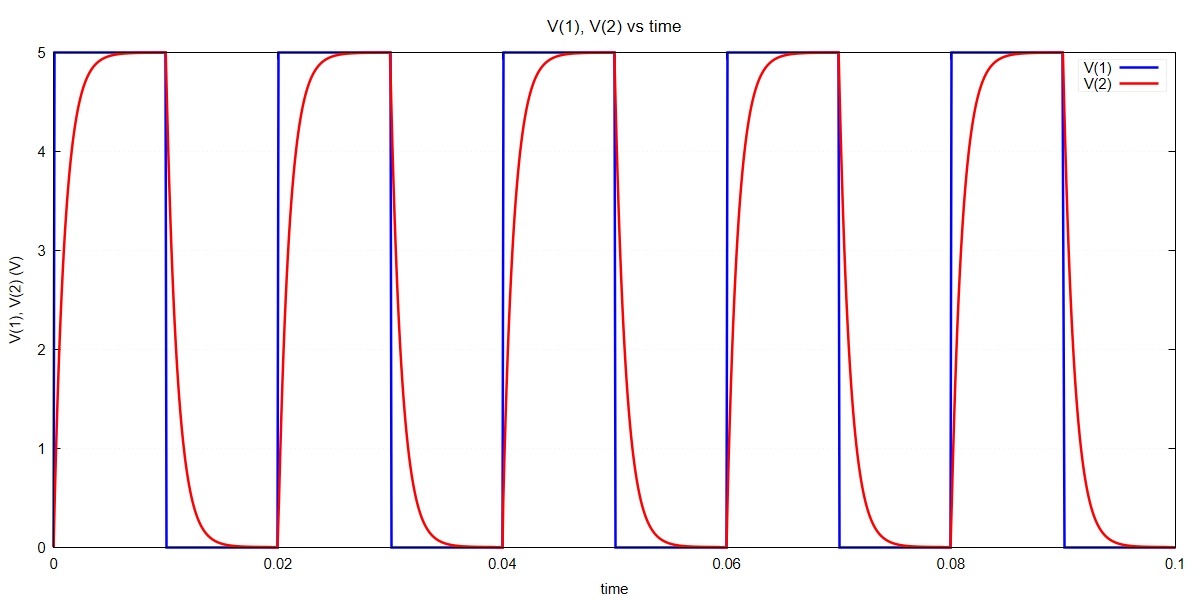
\includegraphics[width=0.75\textwidth]{Figures/ch7/Multiple_signals.png}
  \caption{Transient plot of \texttt{V(1)} and \texttt{V(2)} overlaid on a single panel.}
  \label{fig:tran_single}
\end{figure}

\paragraph{Dual Panel Plot}
\textbf{Command:} \texttt{plot time V(1) I\_branch(1) --out dualpanel.png}\\
\textbf{Description:} Signals with different physical units or extreme magnitude differences are automatically split into stacked sub-panels to prevent visual squashing.

\begin{figure}[H]
  \centering
  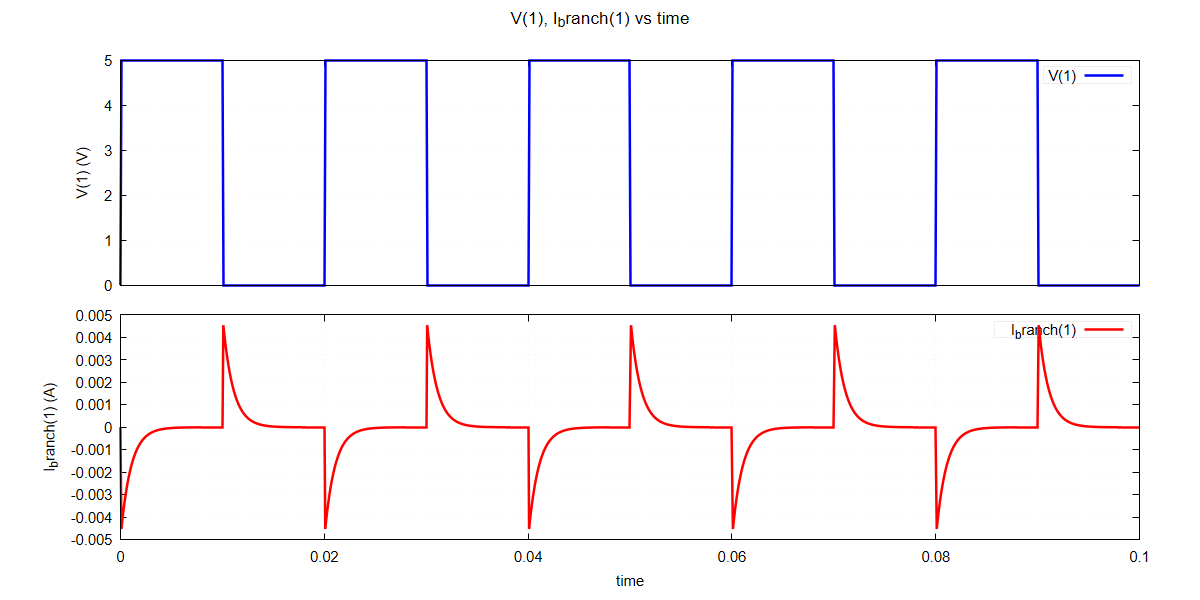
\includegraphics[width=0.75\textwidth]{Figures/ch7/dualpanel.png}
  \caption{Automatic dual-panel split for mixed voltage/current signals.}
  \label{fig:tran_dual}
\end{figure}

% -------------------------------------------------------------------
\subsubsection{AC Analysis Plots}
\label{sssec:ac-plots}
% -------------------------------------------------------------------

\paragraph{Complex Accessors}
\textbf{Command:} \texttt{plot freq\_Hz db(V(2)) --out complex\_Accessors.png}\\
\textbf{Description:} Explicit complex accessors (\texttt{mag}, \texttt{db}, \texttt{ph}, \texttt{re}, \texttt{im}) produce a single-panel plot of the derived quantity on a logarithmic X-axis.

\begin{figure}[H]
  \centering
  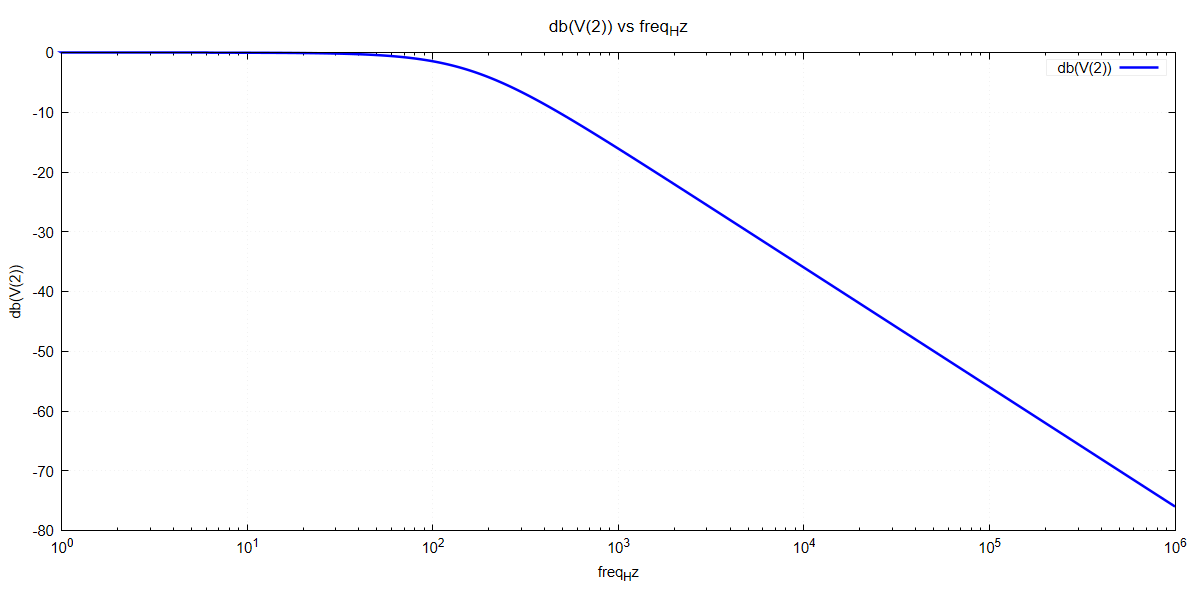
\includegraphics[width=0.75\textwidth]{Figures/ch7/complex_Accessors.png}
  \caption{Single-signal Bode plot showing the magnitude in decibels of \texttt{V(2)}.}
  \label{fig:complex_accessors}
\end{figure}

\paragraph{Full Bode Plots}
\textbf{Command:} \texttt{plot freq\_Hz V(2) --out Full\_bode\_plot.png}\\
\textbf{Description:} A raw complex signal automatically triggers Bode mode, generating a two-panel figure for magnitude (top) and phase (bottom).

\begin{figure}[H]
  \centering
  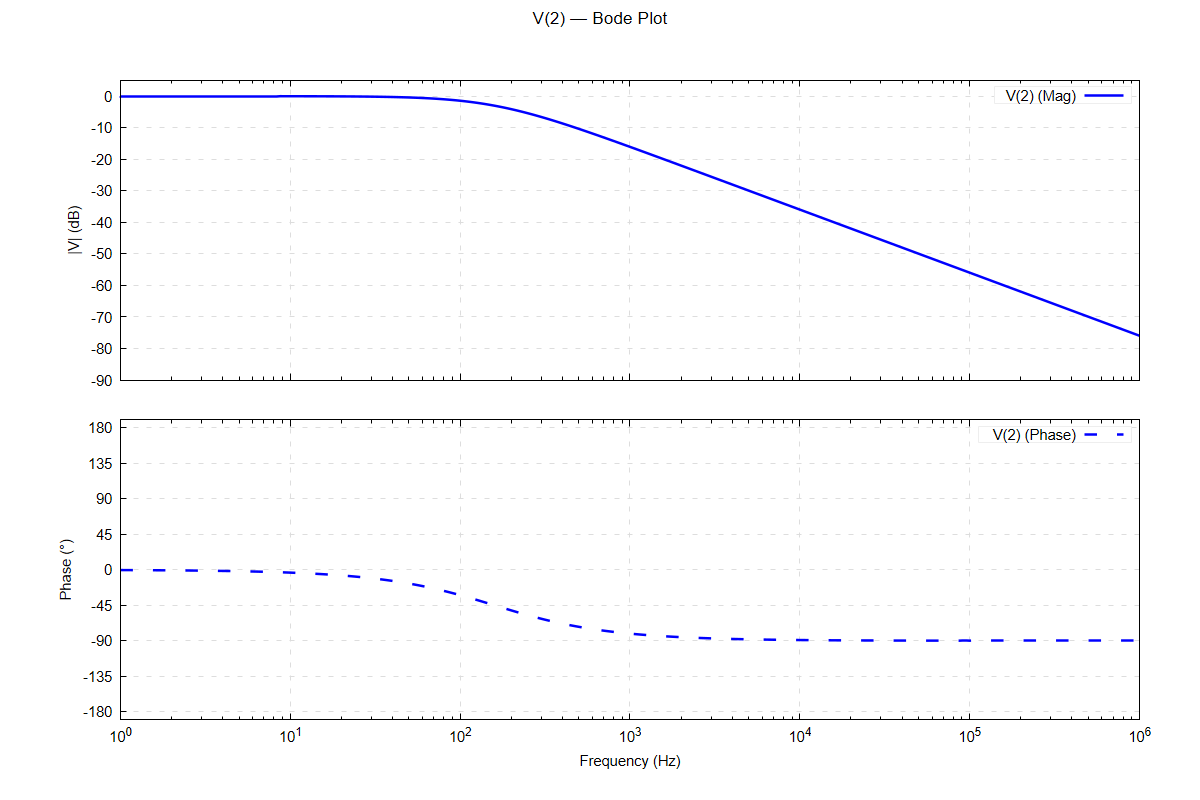
\includegraphics[width=0.75\textwidth]{Figures/ch7/Full_bode_plot.png}
  \caption{One-signal Bode plot for \texttt{V(2)}.}
  \label{fig:full_bode_plot}
\end{figure}

\paragraph{Missing Signal Error}
\textbf{Command:} \texttt{plot time V(99)}\\
\textbf{Description:} If the requested signal does not exist, the engine searches the database, prints an \texttt{[ERROR]} message, and offers fuzzy-matched alternatives such as \texttt{V(9)} or \texttt{V(out)}.

% ---------------------------------------------------------------------------
\section{Software Implementation}
\label{sec:pp-implementation}
% ---------------------------------------------------------------------------
\subsection{Command Interpreter}
\label{subsec:interpreter}

The \texttt{Interpreter} maintains a dispatch table mapping command keyword
strings to command handler objects (\texttt{ICommand}).  Each handler
receives the tokenised input and a shared context (\texttt{InterpreterContext})
containing references to the database and engine objects.

\paragraph{Tokenisation and Suggestions.}
Input lines are split on whitespace and commas, preserving text enclosed in
double quotation marks (\texttt{"..."}).  If an unrecognised command is typed,
a Levenshtein edit distance search suggests commands within a distance of two.
Fuzzy substring search suggests signal names if a signal is not found.

\subsection{UML Diagrams}
\label{sec:pp-uml}
% ---------------------------------------------------------------------------

The class-level design is divided into six logical subsystems for clarity.
The following diagrams illustrate the static structure, composition, and dependencies of each package.

\subsubsection{Application Entry and Core Interpreter}
\label{subsec:uml-entry-interpreter}

This diagram focuses on the top-level wiring of the application.
It includes the \textbf{Application Entry} package (containing the \texttt{Main} class),
the core components of the \textbf{Command Interpreter System}
(specifically \texttt{Interpreter}, \texttt{InterpreterContext}, and \texttt{ConstraintGuard}),
along with the \textbf{Utilities} package (\texttt{intrp\_util} and \texttt{GlobalHelpers})
and the \textbf{Standard Library} exception hierarchy.

\begin{figure}[H]
  \centering
  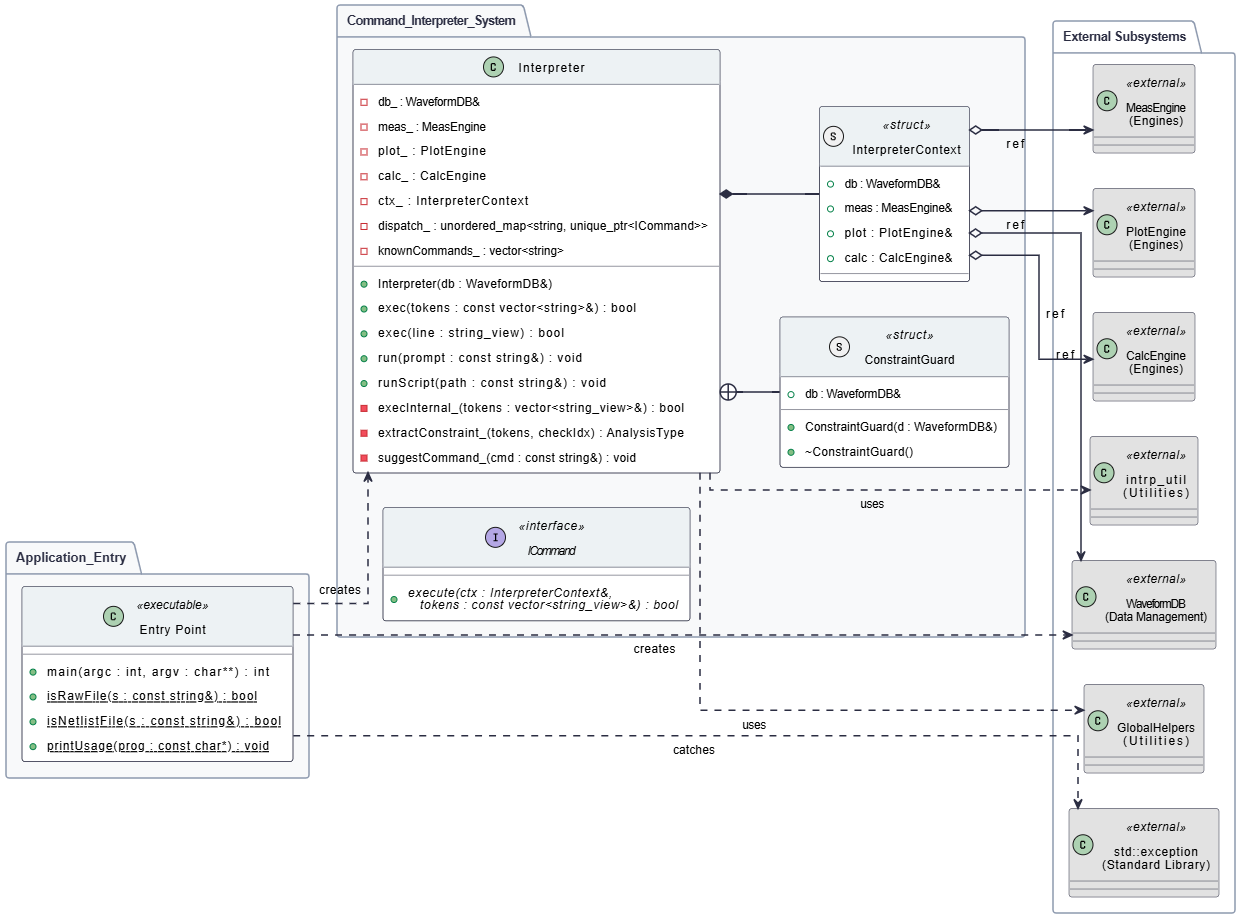
\includegraphics[width=0.75\textwidth]{Figures/ch7/P_UML1.png}
  \caption{Class relationships of the Application Entry Point and the Core Interpreter.}
  \label{fig:UML1}
\end{figure}

Figure~\ref{fig:UML1} presents the application structure. The Interpreter acts as the central coordination component and communicates with the database and analysis modules through InterpreterContext. The command architecture enables independent extension of new analysis features.

\subsubsection{Command Hierarchy}
\label{subsec:uml-commands}

This diagram details the command dispatch system. It shows the \texttt{ICommand}
interface and its concrete implementations grouped by their logical sub-packages:
\textbf{Data Commands} (\texttt{LoadCommand}, \texttt{DbCommand}, \texttt{InfoCommand}, \texttt{ListCommand}, \texttt{PrintCommand}), 
\textbf{Analysis Commands} (\texttt{MeasCommand}, \texttt{CalcCommand}, \texttt{PlotCommand}),
\textbf{File Commands} (\texttt{SourceCommand}, \texttt{ExportCommand}), and
\textbf{Utility Commands} (\texttt{HelpCommand}).

\begin{figure}[H]
  \centering
  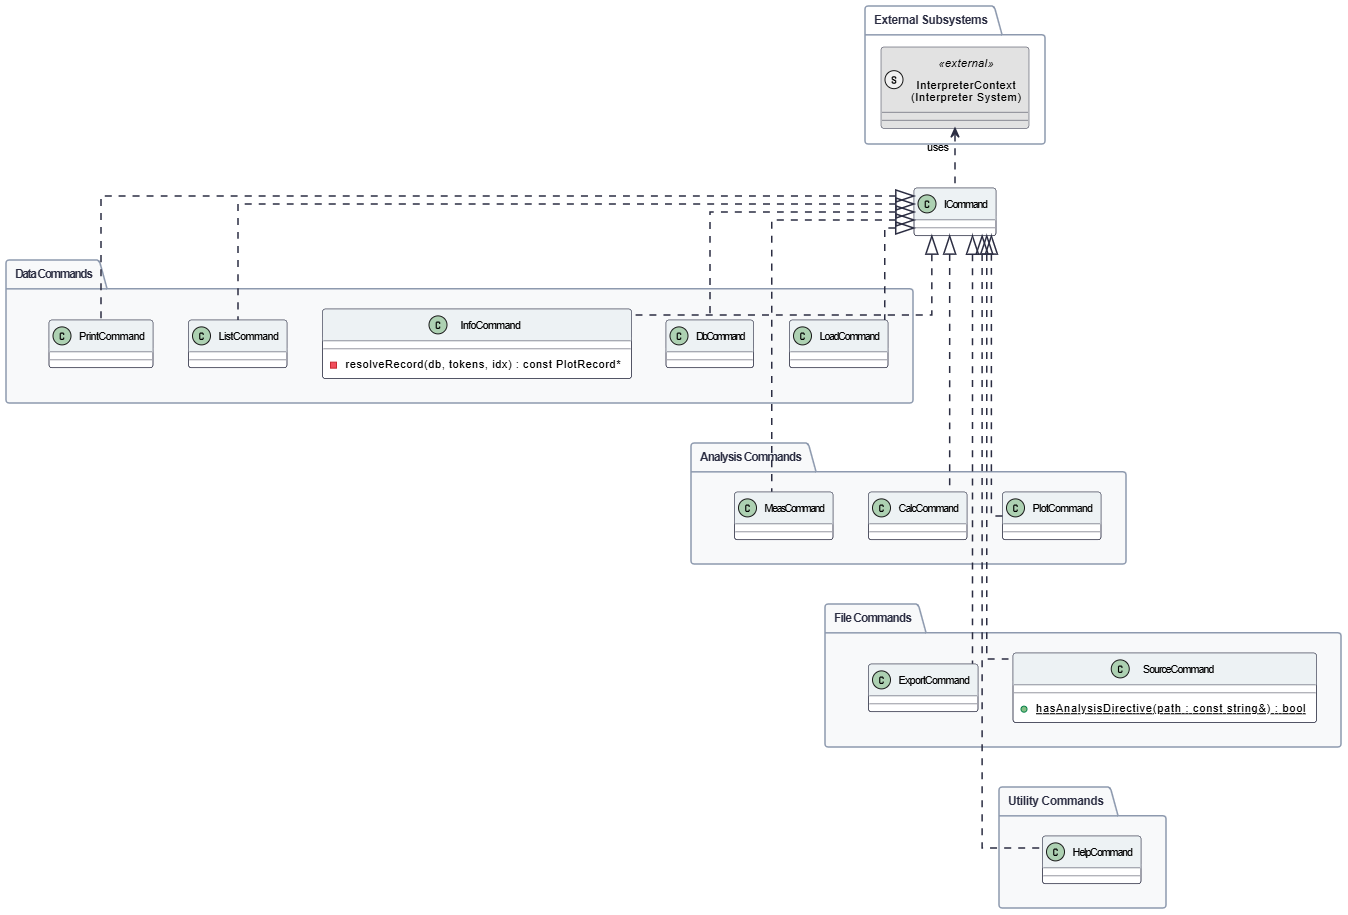
\includegraphics[width=0.75\textwidth]{Figures/ch7/P_UML2.png}
  \caption{Class relationships detailing the Command Dispatch System and Command Hierarchy.}
  \label{fig:UML2}
\end{figure}





\subsubsection{Expression Calculator Engine}
\label{subsec:uml-calc}

This diagram focuses exclusively on the \texttt{CalcEngine} group within the Engines package.
It depicts the \texttt{CalcEngine} class, its inner \texttt{Value} structure,
and the \texttt{CalcResult} struct it produces. 

\begin{figure}[H]
  \centering
  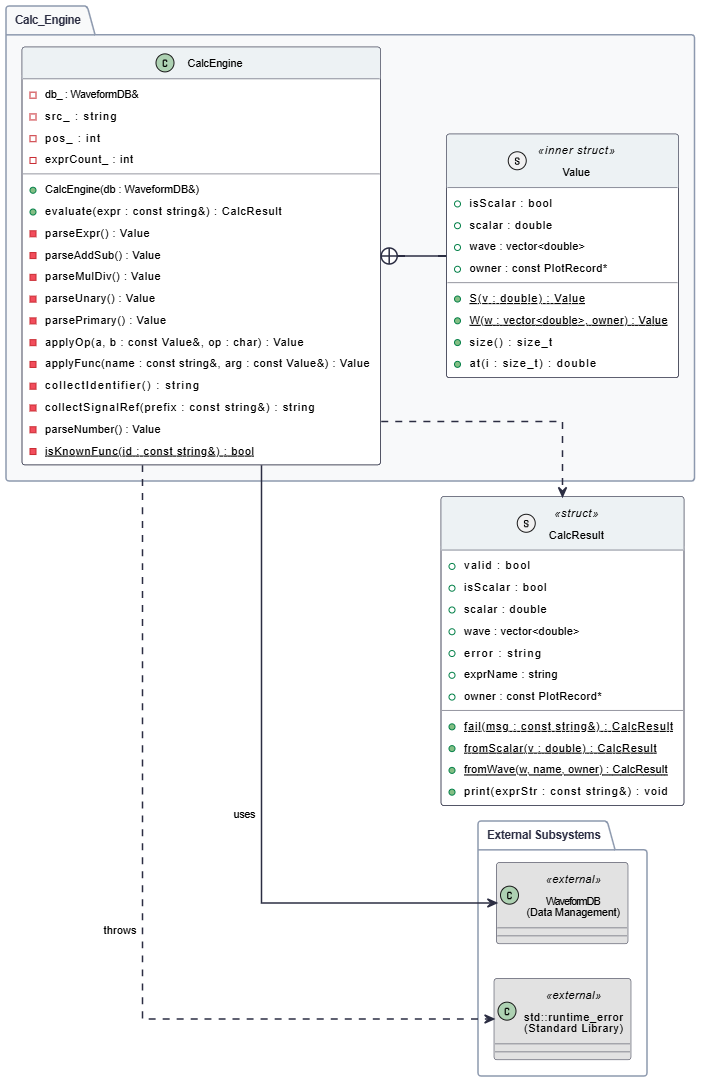
\includegraphics[width=0.75\textwidth]{Figures/ch7/P_UML3.png}
  \caption{Class relationships and internal structures of the Expression Calculator Engine.}
  \label{fig:UML3}
\end{figure}





\subsubsection{Measurement Module and Visualization Module}
\label{subsec:uml-meas-plot}

This diagram covers the remaining components in the Engines package: the
\texttt{MeasEngine} and the \texttt{PlotEngine}. It shows \texttt{MeasEngine}
alongside its \texttt{MeasResult} struct, and the \texttt{PlotEngine} class.

\begin{figure}[H]
  \centering
  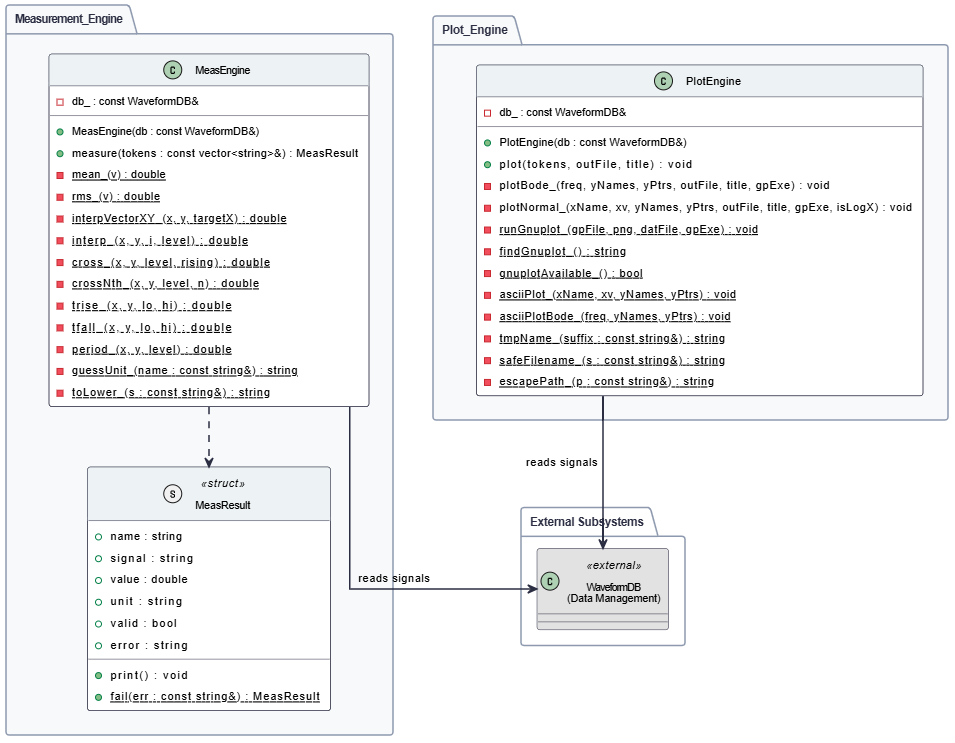
\includegraphics[width=0.75\textwidth]{Figures/ch7/P_UML4.png}
  \caption{Class relationships and dependencies of the measurement and visualization subsystems.}
  \label{fig:UML4}
\end{figure}





\subsubsection{Waveform Database and Data Records}
\label{subsec:uml-waveformdb}

This diagram illustrates the \textbf{Data Management} layer. It includes
the \texttt{WaveformDB} class, the \texttt{PlotRecord} struct it contains, and the
\texttt{AnalysisType} enumeration.

\begin{figure}[H]
  \centering
  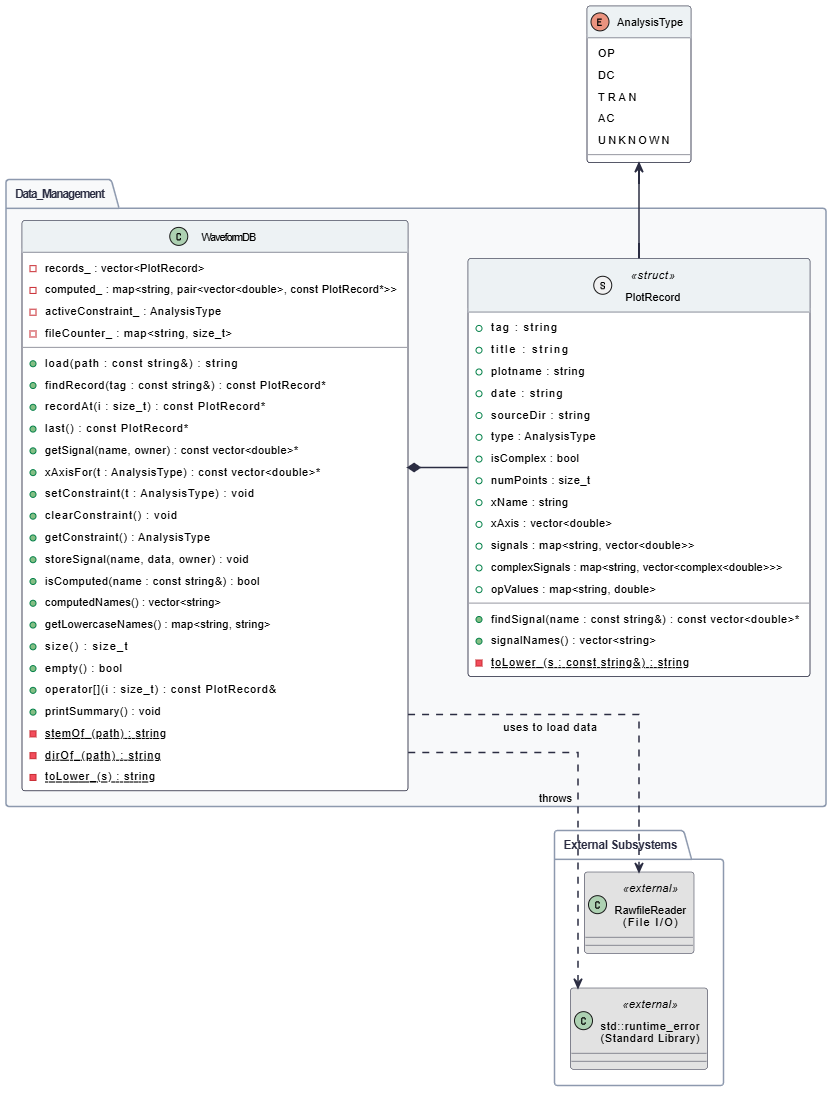
\includegraphics[width=0.75\textwidth]{Figures/ch7/P_UML5.png}
  \caption{Class relationships representing the Waveform Database and Data Management layer.}
  \label{fig:UML5}
\end{figure}





\subsubsection{File I/O Layer}
\label{subsec:uml-fileio}

The final diagram presents the \textbf{File I/O} layer. It shows the
\texttt{RawfileReader} class, the \texttt{RawFile} structure it returns, and the
\texttt{RawSignal} struct representing individual signals inside the file.

\begin{figure}[H]
  \centering
  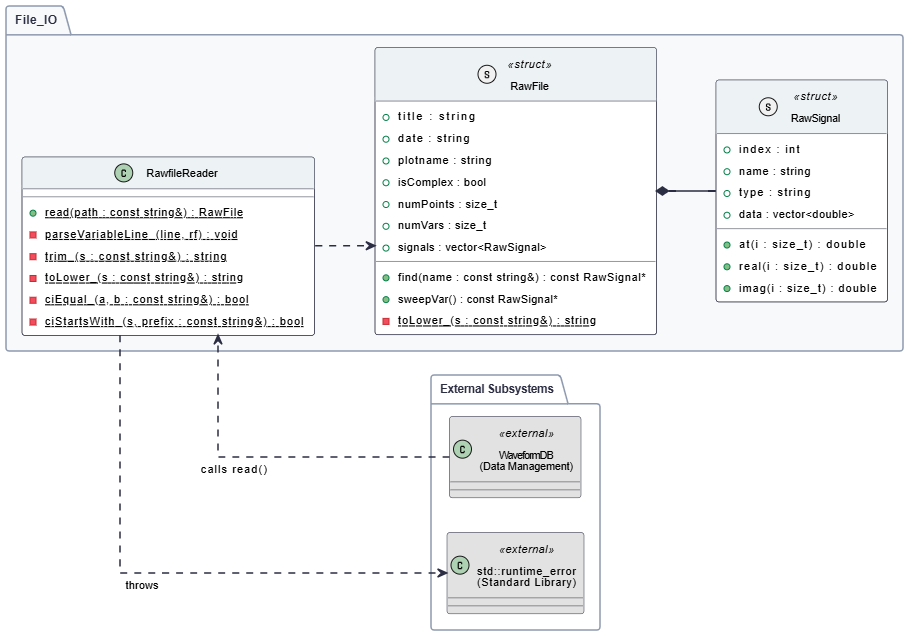
\includegraphics[width=0.75\textwidth]{Figures/ch7/P_UML6.png}
  \caption{Class relationships of the File I/O layer and Rawfile parsing structures.}
  \label{fig:UML6}
\end{figure}





\subsection{Error Handling}
\label{sec:pp-errors}
% ---------------------------------------------------------------------------

Every command performs input validation before accessing data. Error messages
follow a uniform format prefixed with \texttt{[ERROR]}, followed by a description
and a corrective hint. The interactive REPL loop never terminates upon encountering
a command error; it simply prints the error and awaits the next command.

Common handled errors include:
\begin{itemize}
  \item \textbf{No data loaded:} Directs the user to use \texttt{load} or \texttt{source}.
  \item \textbf{Signal not found:} Suggests up to three fuzzy-matched alternatives.
  \item \textbf{Missing X-axis data:} Prevent time-domain measurements on operating-point data.
  \item \textbf{Crossing not found:} Warns if signals do not cross required measurement thresholds.
  \item \textbf{Size mismatch:} Caught during \texttt{calc} or \texttt{plot} when
        waveforms are sourced from disparate simulation results.
\end{itemize}

% ---------------------------------------------------------------------------
\paragraph{Example diagnostics}
\begin{lstlisting}[style=spicerepl]

spice> plot time V(99)

[ERROR] Signal 'V(99)' not found.
Did you mean:
  V(9)
  V(out)
\end{lstlisting}

\begin{lstlisting}[style=spicerepl]
  
spice> plot time V(1) --out

[ERROR] Missing filename after --out.
\end{lstlisting}


% ---------------------------------------------------------------------------
\section{Verification}
\label{sec:pp-verification}
% ---------------------------------------------------------------------------
\subsection{Measurement Verification}
\label{sec:meas-verify}

The measurement subsystem is validated through automated Google~Test
suites, each targeting a distinct category of behaviour.

\begin{itemize}
    \item \textbf{Scalar Correctness:} Computes standard measurements such as
          \texttt{max}, \texttt{min}, \texttt{ptp}, \texttt{avg}, and
          \texttt{rms} via the engine and cross-checks each result
          against a reference value derived independently from the raw
          signal vector using standard library algorithms.

    \item \textbf{Windowed Measurements:} Verifies that the optional \texttt{from}~$t_1$
          \texttt{to}~$t_2$ suffix correctly restricts the computation window.
          An out-of-range window (e.g. \texttt{from 100 to 200}) is verified to return an
          invalid result, confirming proper bounds checking is enforced.

    \item \textbf{Time-Domain Features:} Valid commands such as \texttt{trise},
          \texttt{cross}, \texttt{delay}, and \texttt{find} are confirmed to print a
          numeric assignment without producing \texttt{nan}.
          Invalid commands, such as typos, aperiodic waveforms, or wrong axis names,
          are confirmed to produce an \texttt{[ERROR]} message on \texttt{stderr}.

    \item \textbf{Periodic Signals:} A dedicated sinusoidal and square-wave netlist
          is simulated to verify periodic measurements. Commands like \texttt{freq},
          \texttt{period}, \texttt{rms}, \texttt{ptp}, and \texttt{delay} are verified
          to return correct values on signals that provide sufficient data. Signals
          whose simulation window covers exactly one period are verified to properly
          fail frequency and period measurements with an error, confirming the boundary-condition guard works as expected.
\end{itemize}

% ---------------------------------------------------------------------------
\subsection{Expression Evaluation Verification}
\label{sec:calc-verify}

Four Google~Test suites validate the expression calculator:

\begin{itemize}
    \item \textbf{Scalar arithmetic (T2\_CalcScalar):} Sixteen parameterised
          cases verify pure-scalar expressions including all four operators,
          nested parentheses, unary negation, and all engineering-suffix
          literals. Each result is cross-checked with \texttt{EXPECT\_NEAR}
          to tolerance \texttt{1e-9}.

    \item \textbf{Element-wise wave functions (T2\_CalcWaveFunc):} Twelve
          cases exercise \texttt{abs}, \texttt{neg}, \texttt{sqrt},
          \texttt{exp}, \texttt{sin}, \texttt{cos}, \texttt{tan},
          scalar-broadcast arithmetic, and two-signal operations
          (\texttt{V(1)-V(2)}, \texttt{V(1)+V(2)}, \texttt{V(1)*V(2)}).
          Every sample is verified element-by-element against a
          reference computed directly in C++.

    \item \textbf{Reduction functions (T2\_CalcReduce):} Five cases confirm
          that \texttt{max}, \texttt{min}, \texttt{avg}, \texttt{mean},
          and \texttt{rms} collapse a waveform to the correct scalar.

    \item \textbf{Error handling (T2\_CalcError / T2\_CalcEmpty):}
          Invalid expressions (\texttt{1/0}, unclosed parenthesis,
          trailing operator, unknown function) are each confirmed to
          return \texttt{CalcResult.valid = false}. An empty-string
          input is verified not to throw or crash.
\end{itemize}

% ---------------------------------------------------------------------------
\subsection{Plotting Verification}
\label{sec:plot-verify}

The plotting subsystem is validated through a comprehensive Google~Test
fixture (\texttt{PlotCLITest}) containing more than sixty test cases.
To avoid redundancy, the following table lists the unique representative 
test cases, illustrating the command executed, the expected output, and 
the test status.

\begin{table}[H]
\centering
\caption{CLI and Time-Domain Tests (Cases 1.1 -- 1.27)}
\label{tab:tests-case1}
\footnotesize
\begin{tabularx}{\textwidth}{p{6.5cm} X}
\toprule
\textbf{Command Executed} & \textbf{Actual Output} \\
\midrule
\texttt{plot} & Missing arguments. Emits \texttt{[ERROR]}. \\
\texttt{plot time} & Missing Y signal. Emits \texttt{[ERROR]}. \\
\texttt{plot time V(1) -{}-out case1\_3.png} & Generates PNG plot for \texttt{V(1)}. \\
\texttt{plot time V(2) -{}-out case1\_4.png} & Generates PNG plot for \texttt{V(2)}. \\
\texttt{plot time V(1) V(2) } & Generates shared-axis plot for multiple signals. \\
\texttt{plot time V(1) I\_branch(1) } & Generates dual-panel plot for mixed physical units. \\
\texttt{plot time V(99)} & Signal not found. Emits \texttt{[ERROR]} with suggestions. \\
\texttt{plot time v(1) } & Parses case-insensitively. Generates valid plot. \\
\texttt{plot time V(1) -{}-title "..." } & Generates plot containing custom title. \\
\texttt{plot time V(2) -{}- title "..." } & Malformed flag spacing. Emits \texttt{[ERROR]}. \\

\texttt{plot time V(1) -{}-out} & Missing filename argument. Emits \texttt{[ERROR]}. \\
\texttt{plot time V(1) V(1)} & Detects and plot one signal only if are same signals. \\
\texttt{source ../test\_op.cir} & Loads Operating Point (OP) data successfully. \\
\texttt{list} & Lists all signals loaded in memory. \\
\texttt{plot 1 V(1)} & OP data has no valid X-axis. Emits \texttt{[ERROR]}. \\
\texttt{plot V1 V(1) } & Invalid X-axis literal (\texttt{V1}). Emits \texttt{[ERROR]}. \\
\texttt{plot invalid\_x V(1) } & Unknown X-axis variable. Emits \texttt{[ERROR]}. \\
\texttt{plot time invalid\_y } & Unknown Y-axis variable. Emits \texttt{[ERROR]}. \\
\texttt{plot time V(2)} (gnuplot hidden) & Renders ASCII art plot fallback directly to terminal. \\
\bottomrule
\end{tabularx}
\end{table}

\begin{table}[H]
\centering
\caption{AC Analysis, Bode, and Export Tests (Cases 2.1 -- 2.32)}
\label{tab:tests-case2}
\footnotesize
\begin{tabularx}{\textwidth}{p{6.5cm} X}
\toprule
\textbf{Command Executed} & \textbf{Actual Output} \\
\midrule
\texttt{plot freq\_Hz V(2) } & Detects AC data and generates 2-panel Bode plot. \\
\texttt{plot freq\_Hz V(1) V(2) } & Generates multi-signal Bode plot. \\
\texttt{plot freq\_Hz I\_branch(1) } & Generates Bode plot for current. \\
\texttt{plot freq\_Hz mag(V(2)) } & Generates single-panel magnitude plot. \\
\texttt{plot freq\_Hz db(V(2)) } & Generates single-panel dB plot. \\
\texttt{plot freq\_Hz ph(V(2)) } & Generates single-panel phase plot. \\
\texttt{plot freq\_Hz re(V(2)) } & Generates single-panel real-component plot. \\
\texttt{plot freq\_Hz im(V(2)) } & Generates single-panel imaginary-component plot. \\
\texttt{plot freq\_Hz MAG(v(2)) } & Validates case-insensitivity for accessors. \\
\texttt{plot freq\_Hz mag(V(99)) } & AC signal not found. Emits \texttt{[ERROR] because the tested netlist does not contain node 99}. \\
\texttt{plot freq\_Hz V(2) mag(V(2)) s} & Mixed accessor/raw Bode plotting. Generates plot. \\
\texttt{plot freq\_Hz V(2)} (gnuplot hidden) & Generates ASCII art Bode plot fallback because we hide gnuplot path in test. \\
\texttt{plot freq\_Hz V(2) -{}-out ac\_folder/..} & Validates subfolder path resolution. Generates plot. \\
\bottomrule
\end{tabularx}
\end{table}

Additional engine-level validations (\texttt{DirectEngineValidation}) bypass the 
CLI and call \texttt{PlotEngine::plot()} directly with edge-case token lists 
to guarantee internal guard paths are robust against malformed programmatic input.
% ---------------------------------------------------------------------------
\subsection{Validation Summary}
\label{subsec:validation-summary}

The automated validation suites are summarised below so that the chapter
shows coverage at a glance instead of requiring the reader to inspect every
individual case.

\begin{table}[H]
\centering
\caption{Summary of automated post-processing validation coverage.}
\label{tab:validation-summary}
\small
\begin{tabularx}{\textwidth}{p{3.1cm} p{5cm} X}
\toprule
\textbf{Subsystem} & \textbf{Representative Validation} & \textbf{Outcome} \\
\midrule
Plot engine & PlotCLITest, DirectEngineValidation, and more than sixty CLI cases. & Validated with shared-axis, dual-panel, Bode, ASCII fallback, and export checks. \\
Measurement engine & T2\_MeasTranScalar, T2\_MeasWindowed, MeasTranValidTest, and MeasSinValidTest. & Validated across scalar, windowed, threshold-crossing, and periodic-signal behaviour. \\
Expression engine & T2\_CalcScalar, T2\_CalcWaveFunc, T2\_CalcReduce, and T2\_CalcError. & Validated for scalar arithmetic, waveform broadcasting, reductions, and parser errors. \\
Database and errors & CLI guard paths and signal lookup failures. & Validated for missing data, missing signals, and malformed commands. \\
\bottomrule
\end{tabularx}
\end{table}

\section{Performance Considerations}
\label{sec:pp-performance}

The post-processing engine keeps waveform samples in memory so that repeated
measurements, expression evaluations, and plot requests can reuse the same
loaded data without re-reading the raw file.

For the main operations, the asymptotic cost is linear in the number of
waveform samples:

\[
\begin{aligned}
Load & = O(N) \\
Measurement & = O(N) \\
PlotGeneration & = O(N)
\end{aligned}
\]

where $N$ is the number of waveform samples in the loaded record.

The memory complexity is dominated by waveform storage:

\[
Memory = O(MN)
\]

where $M$ is the number of stored signals and $N$ is the number of samples per signal. The memory requirement grows linearly with both the number of waveforms and the simulation resolution. Therefore, storing multiple simulation records provides faster repeated analysis operations but introduces a memory trade-off for large-scale simulations.




% ---------------------------------------------------------------------------
\section{Summary}
\label{sec:pp-summary}
% ---------------------------------------------------------------------------

In this chapter, the architecture, algorithms, and implementation of the custom post-processing framework were detailed. A modular design was presented, isolating data parsing, in-memory waveform management, and specific analysis engines (measurement, expression evaluation, and plotting). Mathematical models underpinning discrete waveform processing were defined, emphasizing how interpolation and statistical metrics are applied to simulation results.

The command-driven interface was designed to offer an interactive REPL as well as batch-scripting capabilities, providing an intuitive grammar for engineering analysis. The extensive automated verification strategies, encompassing Google Test suites across scalar correctness, expression parsing, and plot generation, ensure the reliability of the system as an EDA tool.

Finally, performance considerations were discussed, showing the computational
complexity of waveform processing and the memory trade-off introduced by
in-memory waveform storage. The proposed architecture provides a scalable
foundation for extending the simulator with additional analysis algorithms
and visualization features.
